\chapter{Introduction}
\label{sec:introduction}

The goal of this thesis proposal is to introduce a unified topology optimization framework that uses the \textbf{L}evel \textbf{S}et \textbf{M}ethod (LSM) to describe the design geometry and the e\textbf{X}tended \textbf{F}inite \textbf{E}lement \textbf{M}ethod (XFEM) to solve the governing equations and measure the performance of the design. The framework will be referred to as the LSM-XFEM optimization method.

Topology optimization approaches (see Sections \ref{sec:optimization} and \ref{sec:intro_topology_optimization}) seek the optimal geometry and/or material layout of a body within a given design domain. Popular schemes, such as density methods (Section \ref{sec:density_topology_approaches}), have been widely applied to topology optimization of different physics, such as structures, fluid dynamics, etc. In structural topology optimization, the density method works by transforming the structural optimization problem into a standard nonlinear program where the design variables are coefficients of the governing equation. These design variables are introduced as the material density of the finite elements. Density approaches cannot describe the physics at the phase interface accurately without extensive mesh refinement. This may lead to unphysical responses (Section \ref{sec:SIMP_discussion}). Therefore, problems that require an accurate description of the boundary conditions at the interface may not be suited for density approaches.  The use of level set methods in topology optimization emerged as an alternative to the density approach. Level set methods (Section \ref{sec:intro_level_set_method}) are able to provide an accurate representation of the layout by dividing the design domain into phase regions, where each region may represent a different physics or a different material, as shown in Figure \ref{fig:level_set_circle_description}.
%
\begin{figure}
	\centering
	\begin{tabularx}{\linewidth}{XX}
		\subfloat[]{
			\label{fig:level_set_circle_func_1}
			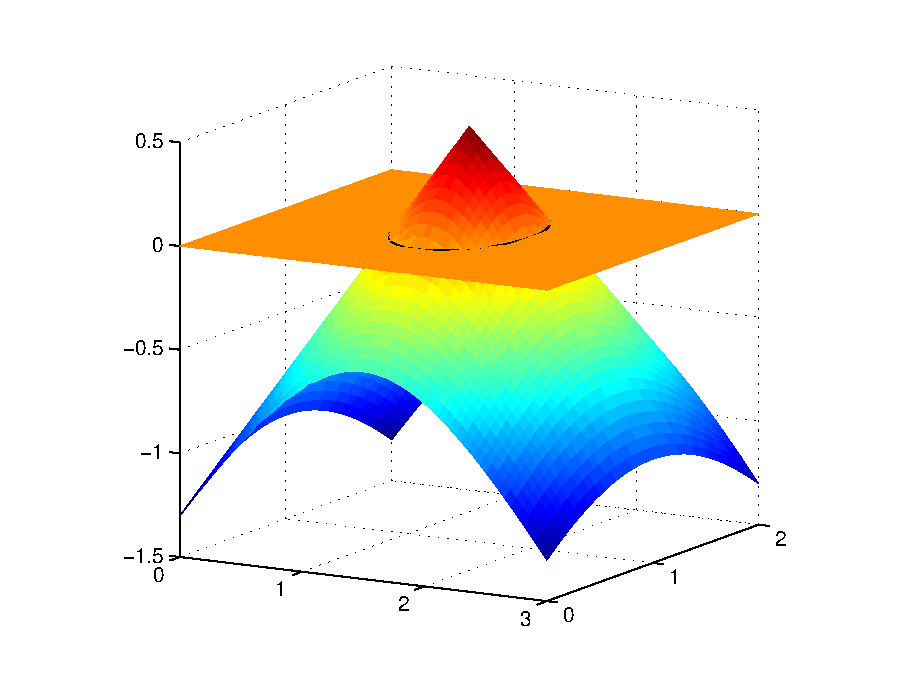
\includegraphics[width=\linewidth]{level_set_circle_func_050.eps}
		} &
		\subfloat[]{
			\label{fig:level_set_circle_domain_1}
			\includegraphics[width=\linewidth]{level_set_circle_domain_050.eps}
		}
	\end{tabularx}
	\caption{The zero level set isolevel of the level set function, $\partial \Omega = \Gamma_{\phi=0}$, in \ref{fig:level_set_circle_func_1} divides the fixed mesh grid into different phase regions in \ref{fig:level_set_circle_domain_1}, where each phase may represent a different material or a different physics.}
	\label{fig:level_set_circle_description}
\end{figure}

To illustrate the differences in the geometry representation between the density and level set methods, consider the ``solid-void'' structural optimization problem presented in Figure \ref{fig:structural_compliance_setup}, where the objective is to minimize the structural compliance by changing the material layout, subject to a maximum volume fraction of 0.5 for the solid phase. The results for both the density and level set approaches are shown in Figure \ref{fig:structural_compliance_comparison}. Notice both designs generate similar truss-like geometries. Figure \ref{fig:structural_compliance_comparison_SIMP} shows how the density method represents the interface between the solid and void materials as intermediate ``grey'' densities, while the level set method in Figure \ref{fig:structural_compliance_comparison_XFEM} describes the geometry by cutting the elements.
%
\begin{figure}[H]
	\centering
	\includegraphics[scale=0.4]{structural_compliance_setup.eps}
	\caption{Setup of a structural topology optimization problem. A mesh of size $3L \times 2L$, with $45 \times 30$ quadrilateral linear elements is anchored to the wall on its left side, and subject to a point load on its right side.}
	\label{fig:structural_compliance_setup}
\end{figure}
%
\begin{figure}[H]
	\centering
	\begin{tabularx}{0.75\linewidth}{X}
		\subfloat[Density method.]{
			\label{fig:structural_compliance_comparison_SIMP}
			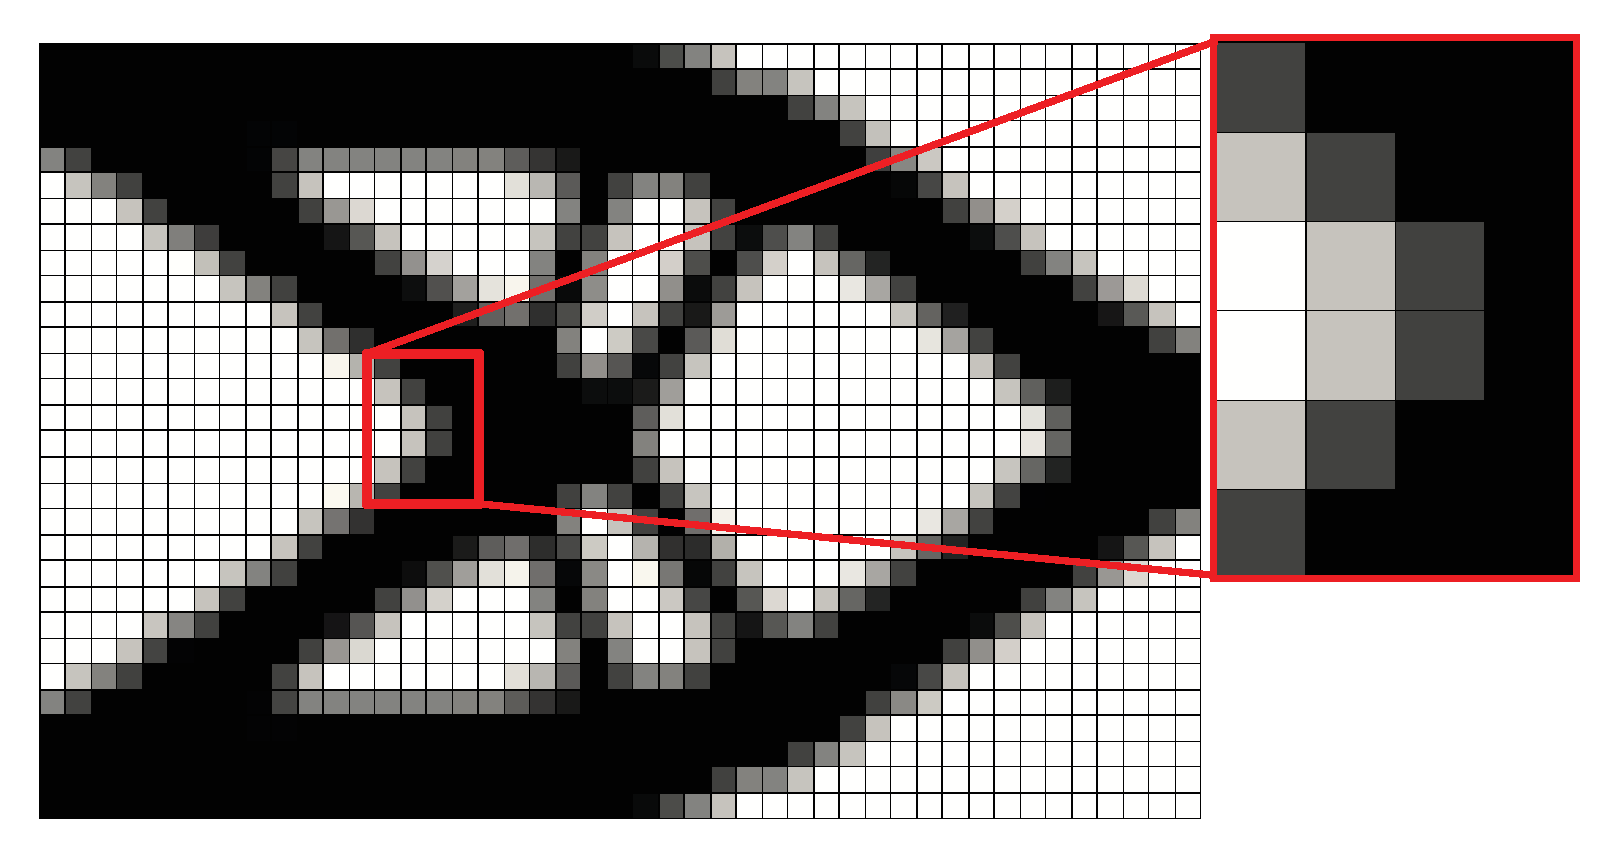
\includegraphics[width=\linewidth]{structural_compliance_comparison_SIMP.eps}
		} \\
		\subfloat[Level set method.]{
			\label{fig:structural_compliance_comparison_XFEM}
			\includegraphics[width=\linewidth]{structural_compliance_comparison_XFEM.eps}
		}
	\end{tabularx}
	\caption{Comparison of the geometry representation of the density and level set methods for a ``solid-void'' structural topology optimization problem.}
	\label{fig:structural_compliance_comparison}
\end{figure}

In the level set method, the material properties of the structural finite elements are interpolated between the void and solid phases, proportional to the volumes of the individual phases. This approach is called Ersatz material interpolation and it is very similar to the interpolation used in density methods. Therefore, it leads to similar issues with regard to enforcing boundary conditions and predicting the physical response along the boundary. The process is illustrated in Figure \ref{fig:ersatz_interpolation}.
%
\begin{figure}[H]
	\centering
	\includegraphics[scale=0.4]{ersatz_interpolation.eps}
	\caption{In an Ersatz material interpolation approach, the material properties of each finite element are interpolated proportional to the volumes of the solid and void phases.}
	\label{fig:ersatz_interpolation}
\end{figure}

An alternative to the Ersatz interpolation is to repeatedly generate new meshes that align with the geometry of the zero level set isolevel, as shown in Figure \ref{fig:remeshing_interpolation}. However, generating an entirely new body fitted
mesh typically suffers from robustness and efficiency, particularly for three dimensional problems. It was also shown by \citep{SMR:00} and \citep{WKG:06} that this method affects the convergence of the optimization process.
%
\begin{figure}[H]
	\centering
	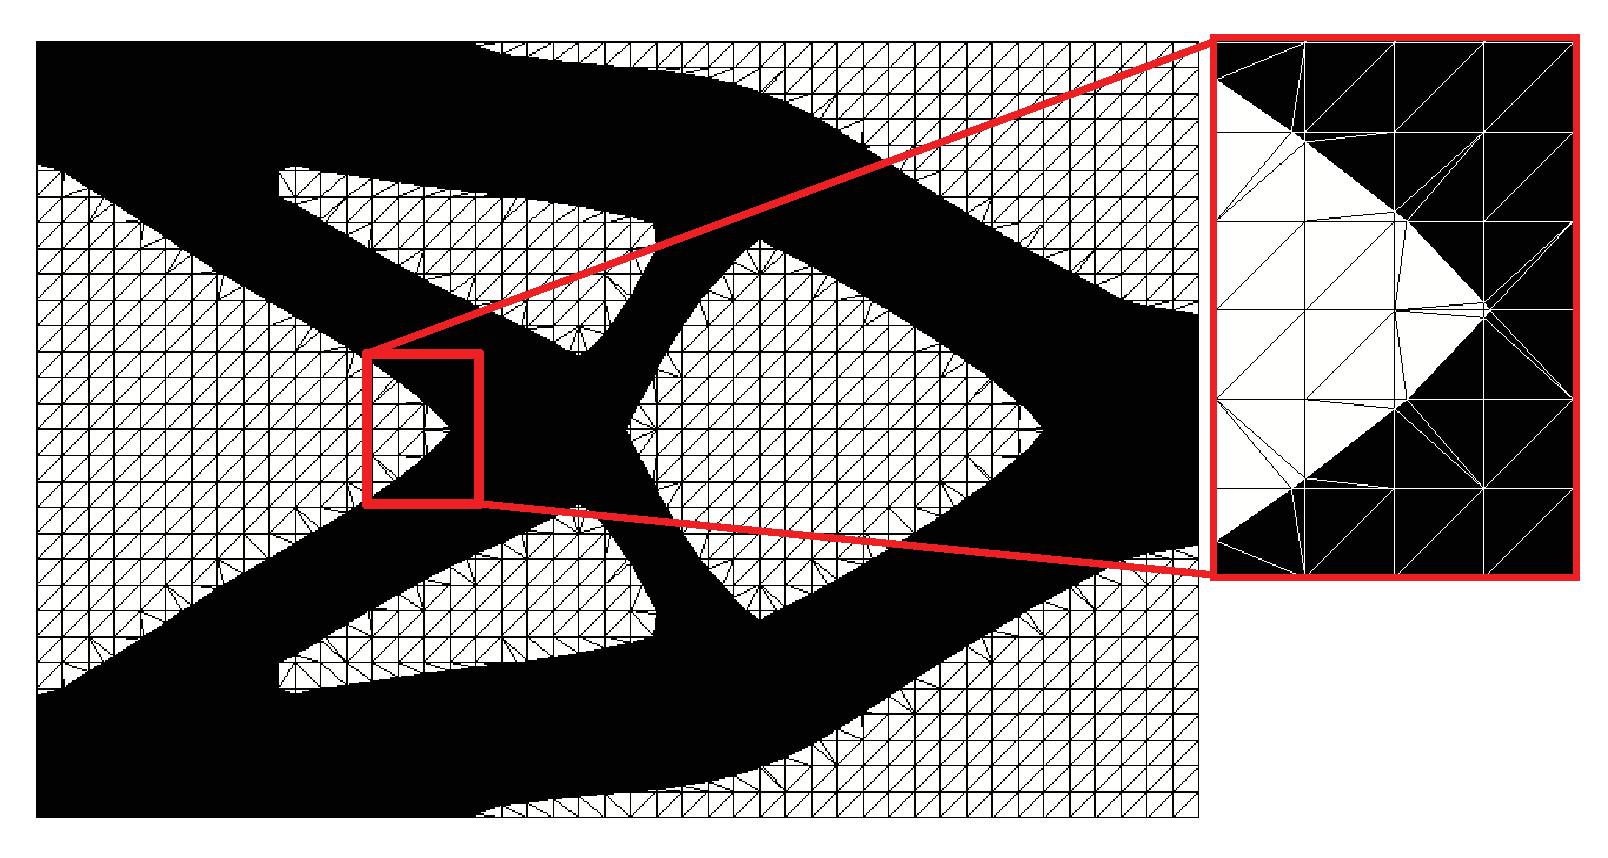
\includegraphics[scale=0.4]{structural_compliance_comparison_remeshing.eps}
	\caption{Remeshing the design domain such that elements align with the zero level set isolevel is an alternative to the Ersatz material interpolation approach.}
	\label{fig:remeshing_interpolation}
\end{figure}

Another approach is used by the XFEM (Section \ref{sec:intro_xfem}). The XFEM is an immersed boundary technique that works on fixed grids, and decomposes the cut elements into subdomains and interfaces that it uses for integration, as shown in Figure \ref{fig:XFEM_interpolation}.
%
\begin{figure}[H]
	\centering
	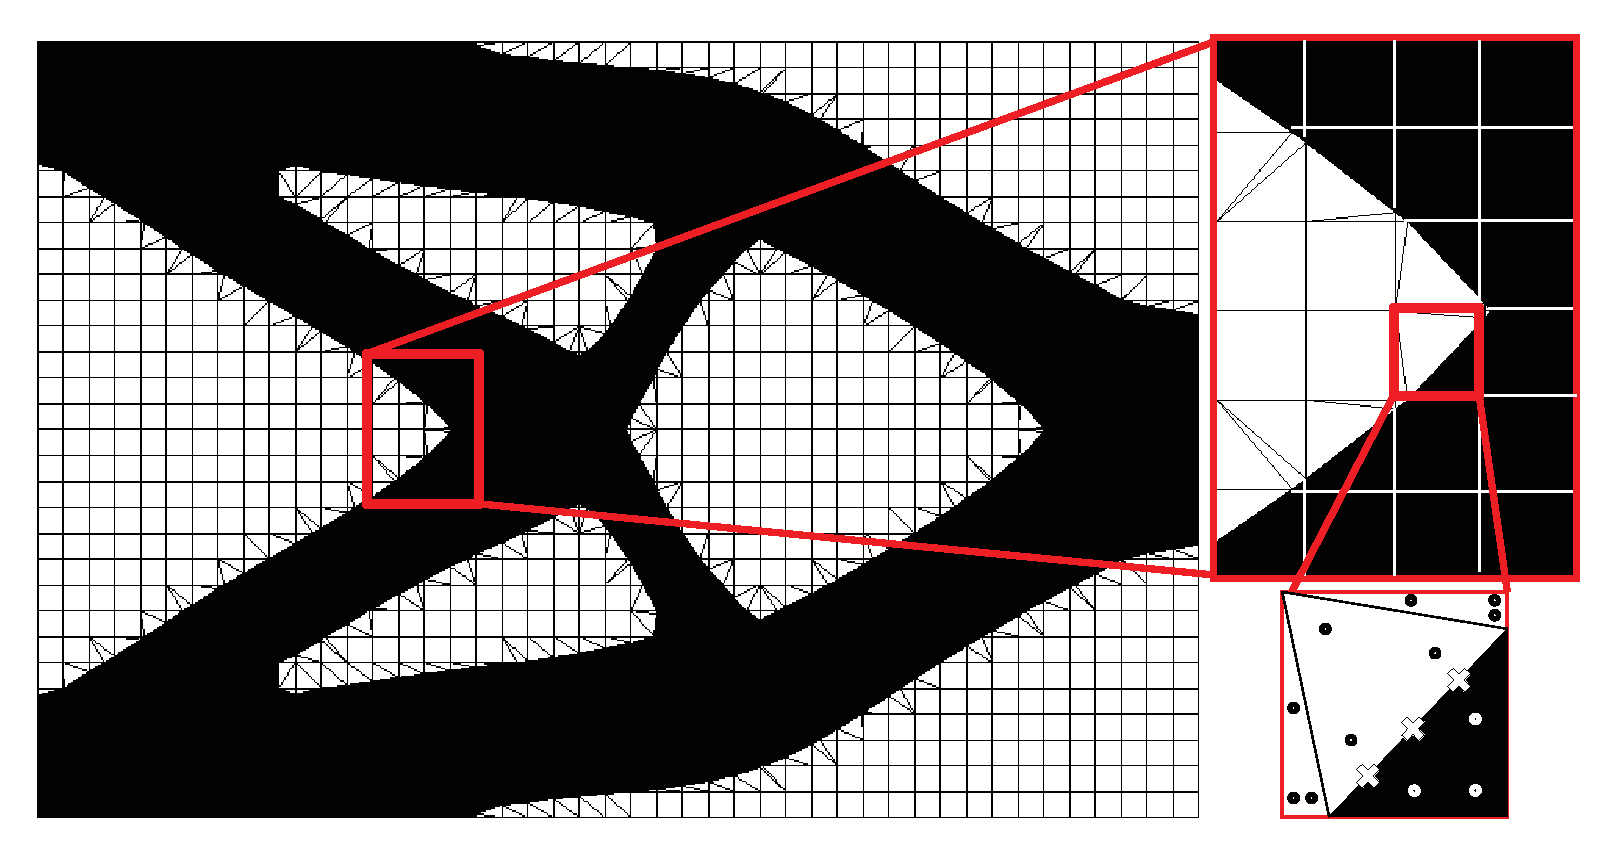
\includegraphics[scale=0.4]{XFEM_interpolation.eps}
	\caption{In the XFEM, the elements cut by the zero level set isolevel are divided into subdomains and interfaces for integration. Circles represent the abscissae for the subdomains, while crosses represent the abscissae for the interface integration.}
	\label{fig:XFEM_interpolation}
\end{figure}

The XFEM enriches the finite element solution space allowing for discontinuities (see Sections \ref{sec:discretization} and \ref{sec:computational-considerations} for details). In this thesis proposal, we will use a Heaviside enrichment strategy, which allows for solution fields with discontinuities $C^{-1}$.

As the topology of the level set function changes, it will occur that a phase subdomain is small enough to cause numerical instabilities in the system, and not lead to convergence. Several approaches have been studied in the literature to try and ameliorate this issue. \citep{LMD+:13} introduced a preconditioner that scales the solution space proportional to the areas of the subdomains. \citep{BH:12,SW:14,SRG+:14} used a ghost penalty formulation to smooth the gradients of the solution at the facets of the cut elements. Both approaches presented favorable results for two dimensional diffusion and incompressible Navier-Stokes flow problems.

Perimeter or curvature measures can be computed at the level set interface using the XFEM. These measures can be introduced into the optimization problem in order to provide a global shape control feature, and prevent the appearance of small floating particles \citep{MM:13}.

This thesis proposal will analyze the characteristics of the proposed LSM-XFEM method as follows:

\begin{enumerate}
	\item \citep{MM:13} studied the XFEM decomposition of the cut elements into subdomains, and the application of multiple enrichment levels in two dimensional problems. Our first hypothesis is that the same approach used by \citep{MM:13} can be extended to three dimensions. Section \ref{sec:a_complete_methodology_for_the_implementation_of_XFEM_inclusive_models} studies the algorithmic details of the approach, and the robustness of the method to describe complex three dimensional geometries using the level set method.

	\item The next question is whether the method can accurately describe the physics at the phase interface without extensive mesh refinement. If so, does it provide an advantage over the interface description provided by the density methods? There are several approaches to approximate the solution at the interface of the level set field, as described in Section \ref{sec:intro_xfem}. We will study the application of stabilized Lagrange multipliers in Section \ref{sec:density_and_level_set_XFEM_schemes_for_topology_optimization_of_3D_structures}, and of the Nitsche method in Section \ref{sec:level_set_XFEM_topology_optimization_of_3D_navier_stokes_and_scalar_transport_problems}.

	\item If the framework can describe complex geometries generated by a level set field, as well as accurately represent the physics at the phase interface, how does it fare overall against density approaches? Section \ref{sec:density_and_level_set_XFEM_schemes_for_topology_optimization_of_3D_structures} applies the framework to three dimensional structural problems, and provides a comprehensive comparison against density methods. The objective is to study convergence rates of the optimization problems, shape control of the optimized geometries, postprocessing capabilities of the methods to generate manufacturable designs, and the effects of providing different initial designs to the optimization process. The hypothesis is that the framework provides a better description of the geometry and material distribution than density methods, and therefore requires coarser meshes which leads to faster computations. Furthermore, it provides the capability to extract surface meshes directly from the level set function and manufacture the designs using three dimensional printing. This feature would be promising for rapid-prototyping.

	\item  In section \ref{sec:preconditioner}, we will expand the scaling preconditioning scheme to structural problems. The preconditioner was previously studied for two dimensional heat conduction problems. The scaling should ameliorate the effects that small intersection regions cause to the solution. In section \ref{sec:level_set_XFEM_topology_optimization_of_3D_navier_stokes_and_scalar_transport_problems}, we will study an alternate approach, the face-oriented ghost-penalty, and its effects on incompressible Navier-Stokes flows. This penalty formulation has been studied in the literature for diffusion and incompressible Navier-Stokes problems, and our hypothesis is that it can be applied in our optimization framework to ensure convergence for three dimensional problems.

	\item Once we can ensure convergence of the solution, the framework should be able to solve a broad range of design engineering problems. In this thesis proposal, we will study structural, incompressible Navier-Stokes flow, and scalar transport problems. These physics will help understand the characteristics, and the capability of the method to be applied to real-world engineering problems. Structural problems are studied in Section \ref{sec:density_and_level_set_XFEM_schemes_for_topology_optimization_of_3D_structures}. Incompressible Navier-Stokes and scalar transport problems are studied in \ref{sec:level_set_XFEM_topology_optimization_of_3D_navier_stokes_and_scalar_transport_problems}.

	\item Controlling the shape of the optimized geometry is important in manufacturing. The effects of using a smoothing filter for the level set field (see Section \ref{sec:intro_level_set_method}) will be studied in Section \ref{sec:feature-size-control}. This filter will also be compared against the density filter (see Section \ref{sec:smoothing_filter}) as a way of controlling the minimum feature size. Regularization techniques applied to the level set interface, such as measuring the curvature and perimeter, may cause different optimized geometries to emerge. The use of these measures and its effects on the finalized design will be studied in Section \ref{sec:topology_optimization_approaches_for_the_curvature_minimization_of_level_set_isocontours}.
\end{enumerate}

The studies proposed above will help us understand the characteristics and capabilities of the framework. The final step is to use this knowledge to study the method in the context of a real-world problem that requires the modeling of a three dimensional incompressible Navier-Stokes flow with a scalar transport field in Section \ref{sec:modeling_of_multiple_scalar_transport_fields_for_an_atomic_layer_deposition_machine}.

The specific objectives of this thesis proposal are then:
\begin{inparaenum}[(i)]
	\item To generate a robust LSM-XFEM topology optimization scheme;
	\item To compare the LSM-XFEM optimization scheme with traditional homogenization methods, such as SIMP, and study the advantages and disadvantages of our formulation;
	\item and to explore the characteristics of the methodology through cases studies in selected applications.
\end{inparaenum}

The layout of this thesis proposal is as follows: Section \ref{sec:introduction} presented the motivation and goals of the study, Section \ref{sec:background} presents an overview of the concepts required to understand this work, Section \ref{sec:a_complete_methodology_for_the_implementation_of_XFEM_inclusive_models} presents the algorithm to implement an XFEM framework in software, Section \ref{sec:density_and_level_set_XFEM_schemes_for_topology_optimization_of_3D_structures} presents the application of the methodology in structural problems, and compares the results to density approaches, Section \ref{sec:level_set_XFEM_topology_optimization_of_3D_navier_stokes_and_scalar_transport_problems} presents the application of the method to incompressible Navier-Stokes flows and scalar transport problems, Section \ref{sec:topology_optimization_approaches_for_the_curvature_minimization_of_level_set_isocontours} studies regularization techniques to improve the manufacturing of the design, Section \ref{sec:modeling_of_multiple_scalar_transport_fields_for_an_atomic_layer_deposition_machine} uses the methodology for a real-world design engineering problem. Finally, Sections \ref{sec:remaining_work} and \ref{sec:main_conclusions} show the remaining work and conclusions of this thesis proposal.

% -----------------------------------------------------------------------------

\chapter{Background}
\label{sec:background}

This chapter presents a brief overview on topology optimization, the level set method, and finite element methods. The information presented in this chapter is sufficient such that the reader can understand the framework in which the thesis is developed, but it is not comprehensive. References are provided for the reader who wishes to see more details on the topics.

% -----------------------------------------------------------------------------

\section{Optimization}
\label{sec:optimization}

An optimization problem is a problem in which you seek to find the best solution from the set of all feasible solutions. There are two categories of optimization problems, and their classification depends on whether the problem variables are continuous or discrete. In this work, we will focus on optimization problems with continuous variables. An optimization problem with discrete variables is known as a combinatorial optimization problem, and the reader is directed to \citep{NW:88} for a review.

The standard form for an optimization problem with continuous variables is:
%
\begin{equation}
\label{eq:optimization_standard_form}
	\begin{aligned}
		&\min_{\mathbf{s}} \mathcal{F}(\mathbf{s}, \mathbf{u}(\mathbf{s})), \\
		&\text{s.t.\,}
		\begin{cases}
			\mathbf{s}, & \text{subject to design constraints}  \ \mathcal{G}_j \leq 0 \text{,}\\
			\mathbf{u}, & \text{solves} \ W= 0 \ \text{for a given $\mathbf{s}$,}
		\end{cases}
	\end{aligned}
\end{equation}
%
where the goal is to minimize some objective functional $\mathcal{F}$ with respect to the vector of design variables $\mathbf{s}$. The design variables are subject to the $j$-th design constraint $\mathcal{G}_j$, which are enforced as an inequality problem. In general, the objective and constraints depend on the optimization variables, $\mathbf{s}$, and the state variables, $\mathbf{u}$. These state variables, $\mathbf{u}$, satisfy the weak form of the equilibrium equation $W$, which is enforced as an equality constraint. By convention, Equation \ref{eq:optimization_standard_form} defines a minimization problem. Maximization problems are handled by placing a negative sign on the objective functional $\mathcal{F}$.

% -----------------------------------------------------------------------------
% Optimization algorithms

There are several optimization algorithms available to update the design variables. For structural optimization problems with non-trivial and multiple constraints, the Method of Moving Asymptotes (MMA) \citep{Svanberg:87}, and its globally convergent counterpart, the Globally Convergent Method of Moving Asymptotes (GCMMA) \citep{Svanberg:02} have become the algorithms of choice. The work of this document will focus on the GCMMA algorithm. For a reference on more advanced mathematical tools, such as thr Sequential Quadratic Programming (SQP), the Sparse Nonlinear OPTimizer (SNOPT) \citep{GMS:02}, or the Interior Point OPTimizer \citep{WBL:06}, the reader is referred to the work of \citep{SM:13}.

% -----------------------------------------------------------------------------
% Design sensititivies

Gradients of the objective functional and design constraints with respect to the design variables are required by the mathematical algorithms specified above. The sensitivities for the optimization problems presented in this document will be computed using the adjoint method \citep{GP:08,YSL:02}.

In the following sections, we will delve into the approaches available to solve the optimization problem.

% -----------------------------------------------------------------------------

\section{Topology optimization}
\label{sec:intro_topology_optimization}

Topology optimization is a type of optimization problem in which you seek the optimal geometry and/or material layout of a body within a given design domain $D$. For example, mathematically we can formulate the following generic topology optimization problem: 
%
\begin{equation}
\label{eq:topology_optimization_generic}
		\min_{\mathbf{s}} \int_{\Omega} f \left( \mathbf{s(\mathbf{x})} \right) d{\Omega}
\end{equation}
%
which, analogous to Equation \ref{eq:optimization_standard_form} is subject to design constraints and equilibrium equations. The goal of the optimization problem is to minimize some objective functional $\int_{\Omega} f \left( \mathbf{s(\mathbf{x})} \right) d{\Omega}$ over the design domain with respect to the design variables $\mathbf{s(\mathbf{x})}$, where $\Omega$ represents the shape of the design. The optimization problem will set the design variables as ``on'' or ``off'' in order to minimize the design objective, while satisfying the design constraints. We can represent a design variable at a point $i$ as ``on'' by setting $s_{i}=1.0$, and ``off'' by $s_{i}=0.0$. A quick example is described in Figures \ref{fig:structural_compliance_setup} and \ref{fig:structural_compliance_example}. Figure \ref{fig:structural_compliance_setup} shows the setup for a topology optimization problem with an objective of minimal compliance and subject to a maximum volume fraction of $0.5$ for the solid phase. Figure \ref{fig:structural_compliance_example} shows the changes in the design, where the design variables at the elements are represented as ``on'' (black) or ``off'' (white) or in-between (grey).
%
\begin{figure}
	\centering
	\begin{tabularx}{\linewidth}{XX}
		\subfloat[Step 0.]{
			\label{fig:structural_compliance_0}
			\includegraphics[width=\linewidth]{structural_compliance_0.eps}
		} &
		\subfloat[Step 5.]{
			\label{fig:structural_compliance_5}
			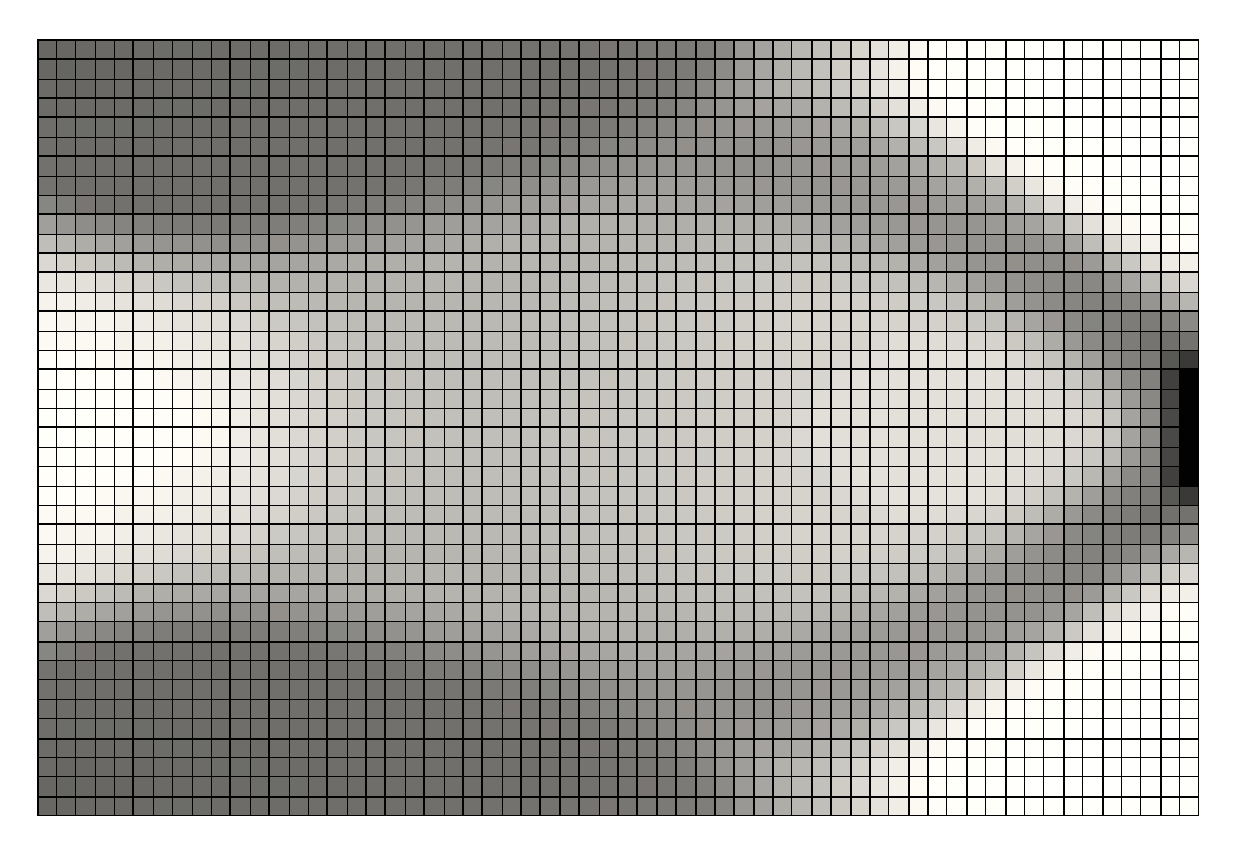
\includegraphics[width=\linewidth]{structural_compliance_5.eps}
		} \\
		\subfloat[Step 10.]{
			\label{fig:structural_compliance_10}
			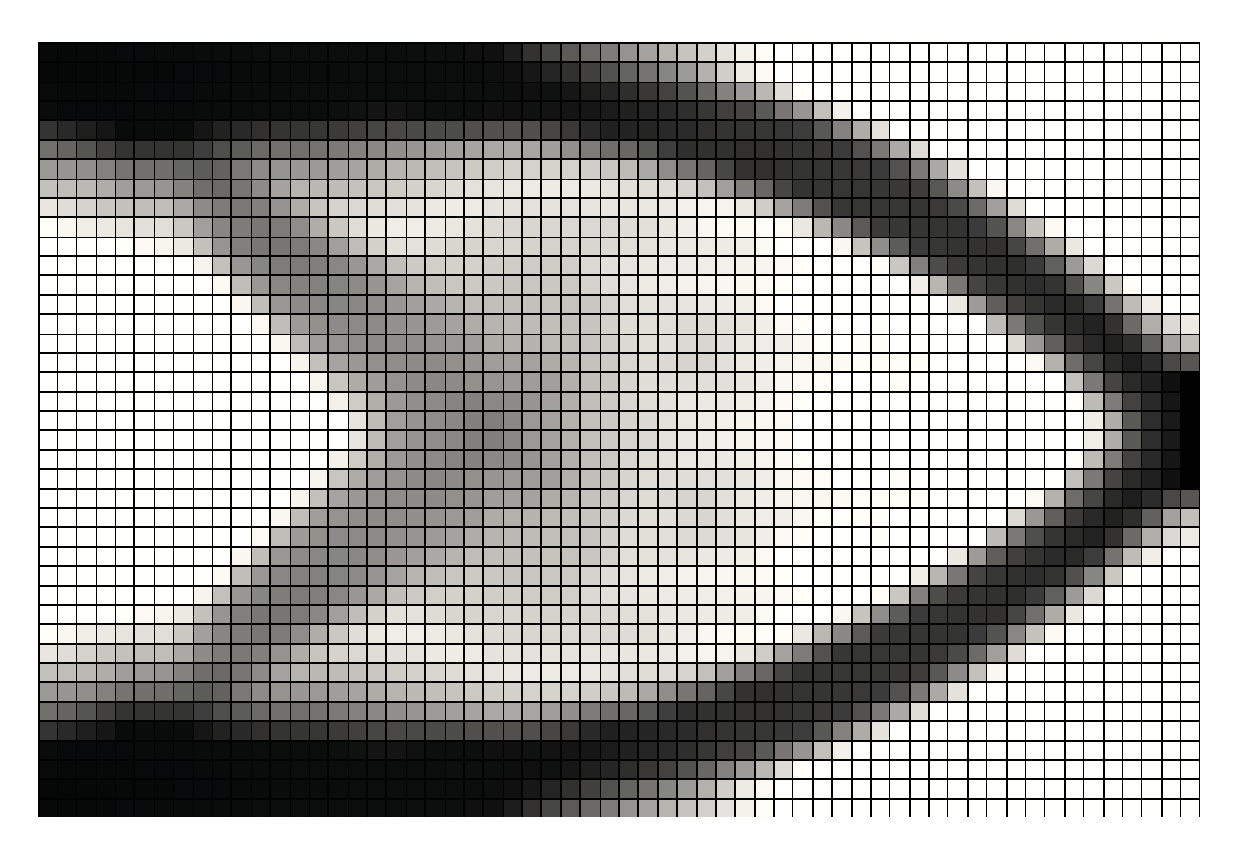
\includegraphics[width=\linewidth]{structural_compliance_10.eps}
		} &
		\subfloat[Step 15.]{
			\label{fig:structural_compliance_15}
			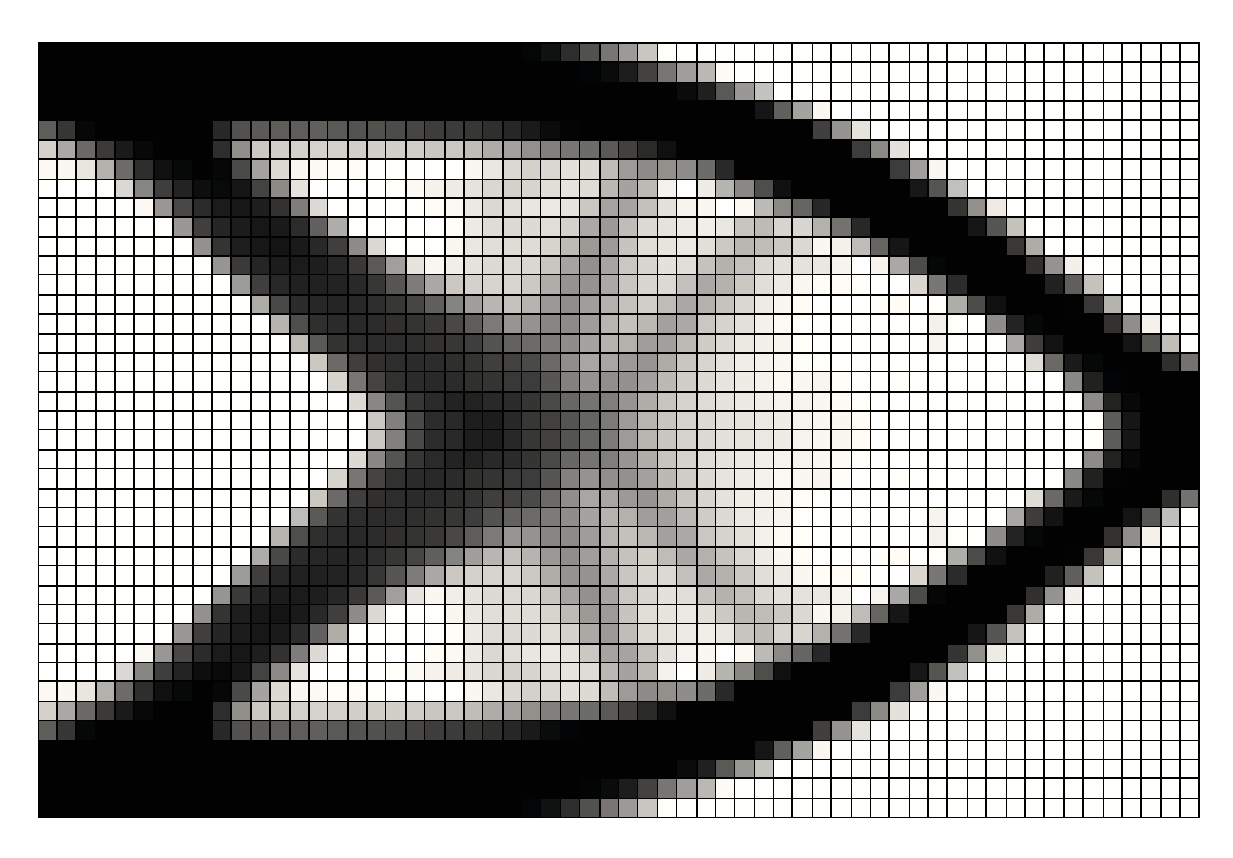
\includegraphics[width=\linewidth]{structural_compliance_15.eps}
		} \\
		\subfloat[Step 25.]{
			\label{fig:structural_compliance_25}
			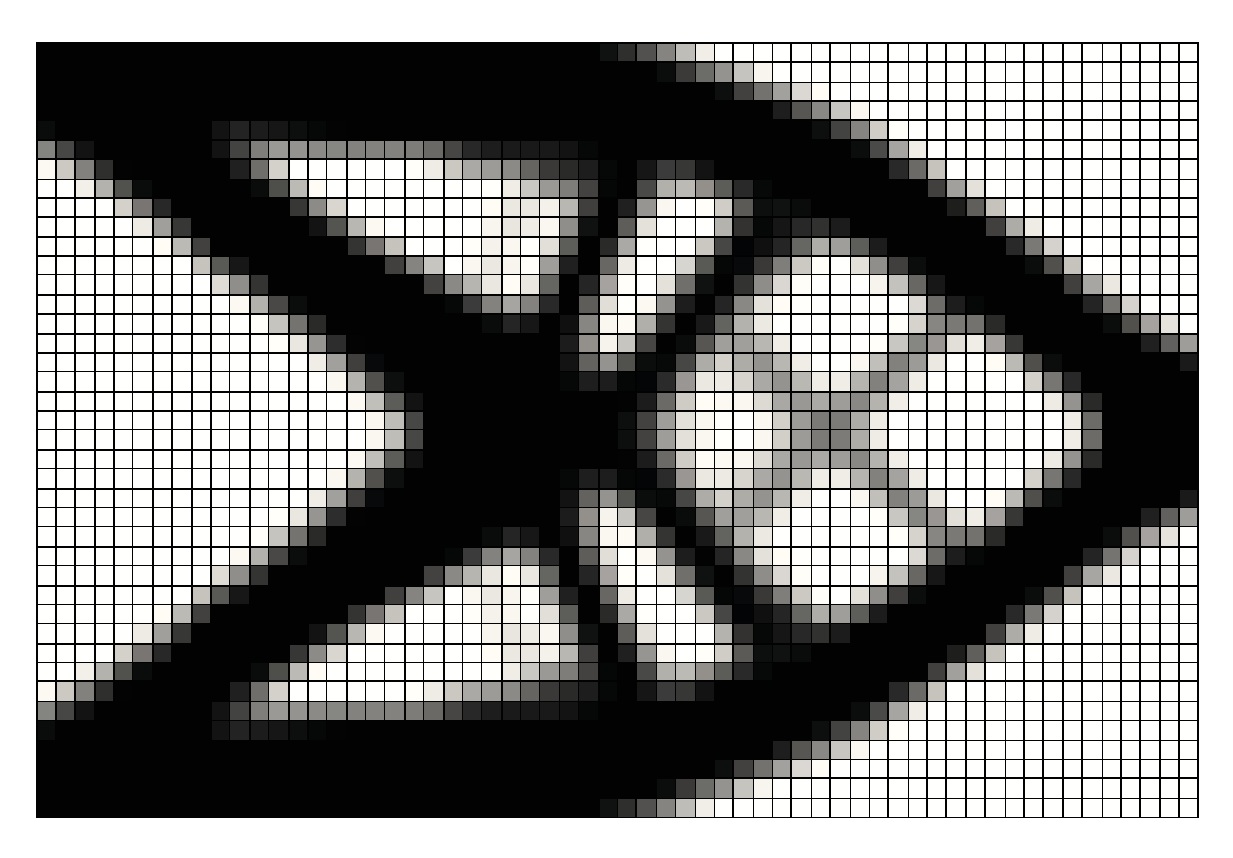
\includegraphics[width=\linewidth]{structural_compliance_25.eps}
		} &
		\subfloat[Step 50.]{
			\label{fig:structural_compliance_50}
			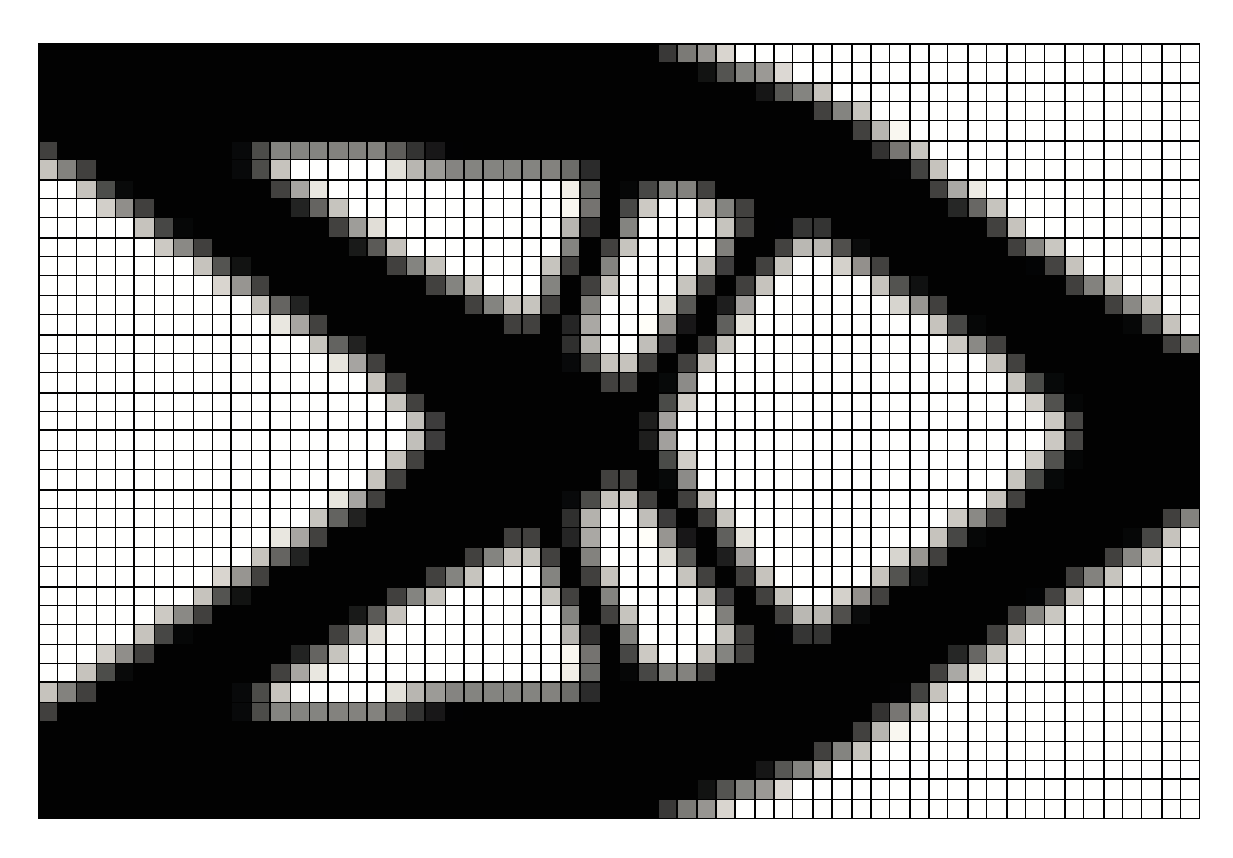
\includegraphics[width=\linewidth]{structural_compliance_50.eps}
		} \\
	\end{tabularx}
	\caption{Progression of the optimization process. Objective is to minimize compliance subject to a maximum volume fraction of 0.5 for the solid phase.}
	\label{fig:structural_compliance_example}
\end{figure}

Topology optimization provides the ability to create designs that are not always intuitive, or to improve on existing designs. Topology optimization methods were initially developed to create conceptual designs in the early stage of the design process \citep{BS:03,Rozvany:09}. It is interesting to note that the earliest recorded paper on topology optimization dates back to 1904, with the work of Australian inventor Michell in the derivation of optimality criteria for least-weight layout of trusses \citep{Michell:04}. And while topology optimization focused for decades on structural design, it has recently found its application in a wide range of physical disciplines \citep{BLO+:05} including acoustics \citep{FAN+:04}, wave propagation \citep{Frenzel:04}, electromagnetics \citep{LGD:09,SHW+:08} and optics \citep{BHF+:04,KOY:05}. For a more detailed review on topology optimization, please refer to \citep{BS:03,EO:01}.

% \footnote{\label{fn:topopt_app}
% At this point, the author recommends you take out your iPhone and iPad and download the best (and ahem... only) structural topology optimization application in the market, TopOpt, from the DTU Mechanical Engineering department. Use this as an exercise to reinforce the concepts explained in this paragraph. Start the application and define a structural problem adding boundary conditions and loads. Before you start the optimization process, try and think of what a good design would be for the problem at hand. Do this for several problems, and compare your intuition to the results of the optimization application. You may realize how helpful topology optimization can be for creating structures with the optimal design.}

% -----------------------------------------------------------------------------
% \subsection{Structural topology optimization}

Structural topology optimization, specifically topology optimization of continuum structures, is in its mathematical nature one of the most challenging optimization problems \citep{BS:03}. However, in 1988, \citep{BK:88} introduced their seminal paper on the homogenization method. In this method, the design domain is assumed to be formed by a material with micro-scale voids, and the topology optimization problem seeks the optimal porosity of the porous medium in order to minimize the objective functional. Due to its effectiveness and simplicity, homogenization-based methods found a lot of applications in structural design, and quickly became the main approach in structural topology optimization \citep{Bendsoe:89}. The homogenization method works by transforming the structural optimization problem into a standard nonlinear program where the design variables are coefficients of the underlying governing equation, and therefore is capable of producing internal holes in the design domain without \textit{a priori} knowledge of them.

% -----------------------------------------------------------------------------

\section{Density topology approaches}
\label{sec:density_topology_approaches}

In 1989, \citet{Bendsoe:89,ZR:91} introduced the most popular of homogenization methods, the ``solid isotropic material with penalization'' (SIMP). In SIMP, the design variables represent the artificial densities, $\rho\left(\mathbf{x}\right)$, of a group of elements in a fixed finite element grid (our design domain $D$) and their material properties are parameterized in terms of a set of material interpolation functions such that intermediate properties are penalized. The typical approach is to assume a value of $\rho=1.0$ represents solid material, while $\rho=0.0$ represents void.

% -----------------------------------------------------------------------------

\subsection{Smoothing filter}
\label{sec:smoothing_filter}

An additional numerical scheme is necessary to smear out numerical instabilities. This is referred to as the filtering method \citep{Sigmund:01a,Sigmund:01b}. For example, in structural topology optimization, the density, rather than being equal to a single variable, can be computed from a linear smoothing filter as follows:

\begin{equation}
	\label{eq:smoothing_filter_SIMP}
	\tilde{\rho}\left(\mathbf{s}\right)=\frac{\sum_{i=1}^{E}w_{i}s_{i}}{\sum_{i=1}^{E}w_{i}}
\end{equation}

with

\begin{equation}
	\label{eq:weight_SIMP}
	w_{i}=\max \left( 0, r_{\rho} - \Vert \mathbf{x}_i - \mathbf{x} \Vert \right)
\end{equation}

where $s_{i}$ is equivalent to an artificial density $\rho$ at a point $\mathbf{x}_{i}$, $\mathbf{x}_{i}$ is the location of the node at which the design variable $i$ is defined, $\tilde{\rho}\left(\mathbf{s}\right)$ is the density at a point $\mathbf{x}$,  $w_{i}$ is the factor of point $\mathbf{x}$ with respect to the design variable $i$, $r_{\rho}$ is the filter radius, and $E$ is the number of elements in the design domain.

The filter in Equation \ref{eq:smoothing_filter_SIMP} prevents the formation of features smaller than $r_{\rho}$, and serves as a minimum feature size control. However, this comes at the cost of forming intermediate densities along the material interface. Methods for smearing out intermediate densities have been proposed by \citep{FJP:05,Sigmund:07,SS:01a}. \citep{GPB:04} proposed a density projection method to reduce the volume occupied by material with intermediate densities. This projection is based on a smoothed Heaviside function and applied to the densities as follows:
%
\begin{equation}
\label{eq:heaviside_density}
		\hat{\rho}\left(\tilde{\rho}\right) = 1-e^{-\beta\tilde{\rho}}+\tilde{\rho}e^{-\beta}
\end{equation}
%
where $\hat{\rho}$ is the projected density, and the parameter $\beta \ge 0$ controls the crispness of the projection. Notice that for $\beta=0$ we recover the original density $\hat{\rho}=\tilde{\rho}$. As we increase $\beta$, more and more intermediate densities are penalized towards the value of 1.0, as shown in Figure \ref{fig:density_heaviside}. Note, however, that if the objective and/or constraints of the optimization problem find the intermediate densities to be benefitial, the optimization algorithm will ignore the effects of this projection scheme. The reader is referred to \citep{GPB:04,GAH:11,Sigmund:07,XCC:10,WLS:11} for more details on projection schemes.
%
\begin{figure}
	\centering
	\includegraphics[scale=0.75]{density_heaviside.eps}
	\caption{The density Heaviside projection for various magnitudes of $\beta$.}
	\label{fig:density_heaviside}
\end{figure}
%
In structural topology optimization, it is important to model the relation between density and stiffness. SIMP models the stiffness proportional to the density in the power $p$, where $p > 1$ \citep{BS:99}, in order to guarantee a well-posed optimization problem \citep{BS:99}. The structural stiffness for a ``solid-void'' problem can then be formulated as:
%
\begin{equation}
\label{eq:structural_stiffness}
		E\left(\mathbf{x}\right) = \hat{\rho} ^ p E_{0}
\end{equation}
%
where $E_{0}$ is the initial structural stiffness of the material. Typically, the parameter $p$ is set to 1, and then increased as the optimization progresses \citep{RZS:94}; this is the so-called continuation method \citep{SP:98}. It was shown that if one uses $p > 3$, we recover a black-and-white binary-like material distribution \citep{BS:03}. That is why the density approach has been referred to as a \textit{pixelated} geometric model.

% -----------------------------------------------------------------------------
% Multimaterial SIMP
% \subsection{Multimaterial SIMP}

The SIMP method can be expanded to model a multi-material optimization problem. For example, applying a ``rule of mixture'', we can model a two-phase material in structural topology optimization by modifying Equation \ref{eq:structural_stiffness} as:

\begin{equation}
	\label{eq:two_phase_stiffness}
	E\left(x\right) = \hat{\rho} ^ p E_{A} + \left( 1 - \hat{\rho} ^ p \right) E_{B}
\end{equation}

where $E_{A}$ represents the stiffness of material ``A'', and $E_{B}$ represents the stiffness of material ``B''. Notice that if we model the material phase ``B'' as void, and set $E_{B}=0$ we recover the original equation from \ref{eq:structural_stiffness}. This method uses a single design variable field to model up to two different materials.

For a three-phase or more material optimization problem, we require an extended power law interpolation with multiple design variable fields (i.e. $\mathbf{s}_{1}$, $\mathbf{s}_{2}$, etc.), as shown in \citep{WW:04c,PS:14}. In general, the SIMP method requires $\left( n - 1 \right)$ design variable fields for $n$ distinct material phases \citep{WW:04c}.

% -----------------------------------------------------------------------------

\subsection{Density methods applied to fluid dynamics}
\label{sec:intro_density_fluid_dynamics}

Several applications require finding the optimal geometries of systems to improve the performance of internal and external flows \citep{Maute:14}. Adopting the concept of density methods, \citep{BP:03} extended the methodology to fluid related problems. They modeled the influence of a wall or body in the fluid flow by representing it as a body force in the incompressible Navier-Stokes equations as:
%
\begin{equation}
	\label{eq:navier_stokes}
	\rho^{f} \left( \frac{\partial v_{i}}{\partial t} + v_{j} \frac{\partial v_{i}}{\partial x_{j}} \right) = \frac{\partial}{\partial x_{j}} \left( -p \delta_{ij} + \mu^{f} \left( \frac{\partial v_{j}}{\partial x_{i}} + \frac{\partial v_{i}}{\partial x_{j}} \right) \right) + f_{i}
\end{equation}
%
\begin{equation}
	\label{eq:divergence_stokes}
	\frac{\partial v_{i}}{\partial x_{i}} = 0
\end{equation}
%
where $\rho^{f}$ is the fluid density, $v_{i}$ is the velocity along the spatial dimension $i$, $p$ is the fluid mechanical pressure, $\mu^{f}$ is the fluid dynamic viscosity, and $f_{i}$ is the force exerted by the porous media:
%
\begin{equation}
	\label{eq:brinkman_force}
	f_{i} = - \alpha v_{i}
\end{equation}
%
This methodology is referred to as the Brinkman penalization. Similar to structural topology optimization problems, we set the design variables, $\mathbf{s}$, to represent the fluid fraction at a point of the design domain, and set $\mathbf{s}=\gamma=\gamma \left( \mathbf{x} \right)$, where $\left( 0 \le \gamma \le 1 \right)$. Typically, $\gamma = 1$ represents the fluid domain, and $\gamma=0$ represents the solid domain.

The coefficient $\alpha$ can be interpolated from the design variables as:
%
\begin{equation}
	\label{eq:alpha_linear}
	\alpha = \alpha_{max} \gamma
\end{equation}
%
The parameter $\alpha_{max}$ should be large enough such that the term $\mathbf{f}$ in Equation \ref{eq:navier_stokes} sufficiently penalizes the flow to $\mathbf{u}=0$. \citep{KMK:12} set $\alpha_{max}$ to:
%
\begin{equation}
	\label{eq:alpha_max}
	\alpha_{max} = \left( 1 + \frac{1}{Re} \right) \chi
\end{equation}
%
where $Re$ is the Reynolds number, and $\chi$ is set to a very large value, i.e. $10^4$.

However, this linear interpolation causes large gradients in the fluid flow, which cause numerical issues and may lead to the optimization problem converging to a local minimum. \citep{BP:03} introduced a convex interpolation:
%
\begin{equation}
	\label{eq:alpha_interpolation}
	\alpha \left( \mathbf{x} \right) = \alpha \left( \gamma \left( \mathbf{x} \right) \right) = \alpha_{max} + \gamma \left( \alpha_{min} - \alpha_{max} \right) \frac{1 + \alpha_{p}}{\gamma + \alpha_{p}}
\end{equation}
%
Figure \ref{fig:alpha_convex} shows the influence of the perimeter $\alpha_{p}$. In general, we want to choose $\alpha_{p}$ to be as low as possible, but high enough to prevent intermediate porosities from showing up in the optimization process. In the work of \citep{KM:11}, $\alpha_{p}$ was chosen to be 0.01 with favorable results. $\alpha_{min}$ is set to zero, such that at its minimum, $\alpha=0$ recovers the original Navier-Stokes equations.
%
\begin{figure}
	\centering
	\includegraphics[scale=0.75]{alpha_convex.eps}
	\caption{Influence of the interpolation penalty $\alpha_{p}$.}
	\label{fig:alpha_convex}
\end{figure}
%
For more details on topology optimization of Stokes and Navier-Stokes flows, the reader is referred to \citep{Maute:14}.

% -----------------------------------------------------------------------------

\subsection{Discussion of the SIMP approach}
\label{sec:SIMP_discussion}

The concept of relating some artificial densities to the stiffness in structural problems can be expanded to other physics disciplines. The SIMP method can be used the describe material properties in thermal conductivity, magnetic permeability, porosity, etc.; and therefore, it found its way to a wide range of applications. The method requires a relatively small amount of iterations in order for the optimization problem to converge to an optimal design (at least for ``solid-void'' problems). SIMP has this capability because it operates on the entire design domain and not only on the boundaries; therefore, it does not suffer from localization effects. The approach is also suitable for a wide combination of design constraints, multiple load conditions, and extremely large (often 3D) systems. The educational article by \citet{Sigmund:01b} detailing a 99-line SIMP-code implemented in Matlab, as well as his web-based topology optimization program \citep{TS:01}\footnote{The software is now available on iOS phones and tablets.} played an important role in the acceptance of the SIMP method in both the academic and industry communities. Virtually all industrial optimization software uses the SIMP method as their optimization method of choice due to its ease of implementation.

% -----------------------------------------------------------------------------
% What are the disadvantages?

The SIMP method typically describes the interface between the different material domains either by using intermediate densities or by discrete material distributions, which may lead to jagged boundaries. In both cases, the representation of the interface is not precise, and therefore, the enforcement of boundary conditions at the interface is hindered. This may result in non-physical responses, such as premature yielding \citep{MSR:98} in structural mechanics, fluid flow penetrating solid material in low Reynolds number flow \citep{KPM:11}, and scalar fields diffusing through solid material at low P\'{e}clet number flow \citep{MPY+:12}. This issue can be mitigated by representing the material interface more accurately either by mesh refinement or adaptive re-meshing \citep{MR:95,MR:97}. However, for problems that require an accurate geometrical description of the interface, such as stresses in elasticity, boundary layer problems in fluids and skin-depth issues in electromagnetics, SIMP (and other material interpolation methods) will fail due to the jagged edges obscuring the physics \citep{ES:11,YNK+:11}.

Using material interpolation to address multi-material optimization problems is not a physics-based technique, and has been shown to violate the Hashin-Shtrikman bounds for low values of $\rho$ and large values of $p$ \citep{HS:62}. Furthermore, modeling multiple material phases can become complicated \citep{YA:01} and lead to slow convergence due to the larger number of iterations, as shown in \citep{VM:14}.

% -----------------------------------------------------------------------------
% Level set method

\section{Level set method}
\label{sec:intro_level_set_method}

The level set method applied to topology optimization arose as a technique capable of overcoming some of the shortcomings of the density approach. The main advantage of the method is that it allows for the description of complex geometries and the variation of the shape and topology of our design without introducing intermediate materials. A level set approach is a \textit{region-based} model with explicit boundaries, in contrast to the \textit{pixelated} model of the density method \citep{WW:04c}.

The level set method was first used to implicitly represent a structural boundary by \citep{OS:88}. Since then, it has been applied extensively in the field of imaging and computer visions \citep{OP:03}. The level set method eventually found its way to topology optimization, as the technique is well suited for the task: level set functions can form holes, split into multiple pieces, or merge with other level set functions \citep{WW:04c,AJT:02,OS:88}. 

The basic idea behind using the level set method to represent a shape boundary $\Gamma = \partial \Omega$ is to express a curve or surface as the zero level set of a higher dimensional implicit function $\phi$, as shown in Figures \ref{fig:level_set_circle_func_025}, \ref{fig:level_set_circle_func_050}, and \ref{fig:level_set_circle_func_075}, such that:
%
\begin{equation}
	\centering
	\label{eq:isolevel}
	\Gamma = \lbrace \mathbf{x} : \phi\left(\mathbf{x}\right) = 0 \rbrace
\end{equation}
%
Then we can divide the design domain into phase regions as:
%
\begin{equation}
	\centering
	\label{eq:level_set_regions}
	\begin{split}
		\phi\left(\mathbf{x}\right) > 0 & \quad \forall \mathbf{x} \in \Omega \backslash \partial \Omega \text{ (inside the region)} \\
		\phi\left(\mathbf{x}\right) = 0 & \quad \forall \mathbf{x} \in \partial \Omega \text{ (on the boundary)} \\
		\phi\left(\mathbf{x}\right) < 0 & \quad \forall \mathbf{x} \in D \backslash \Omega \text{ (outside the region)}
	\end{split}
\end{equation}
%
where $D$ represents the design domain, either bounded or unbounded, and contains all possible admissible shapes of $\Omega$, as shown in Figures \ref{fig:level_set_circle_domain_025}, \ref{fig:level_set_circle_domain_050}, and \ref{fig:level_set_circle_domain_075}. Each phase region may represent a different material \citep{AJT:02,WW:04c,OS:01,SW:00} or a different physics \citep{LCB:06,GW:08}. In the work of this thesis, the level set method is discretized with a finite element mesh.
%
\begin{figure}
	\centering
	\begin{tabularx}{\linewidth}{XX}
		\subfloat[]{
			\label{fig:level_set_circle_domain_025}
			\includegraphics[width=\linewidth]{level_set_circles_1.eps}
		} &
		\subfloat[]{
			\label{fig:level_set_circle_func_025}
			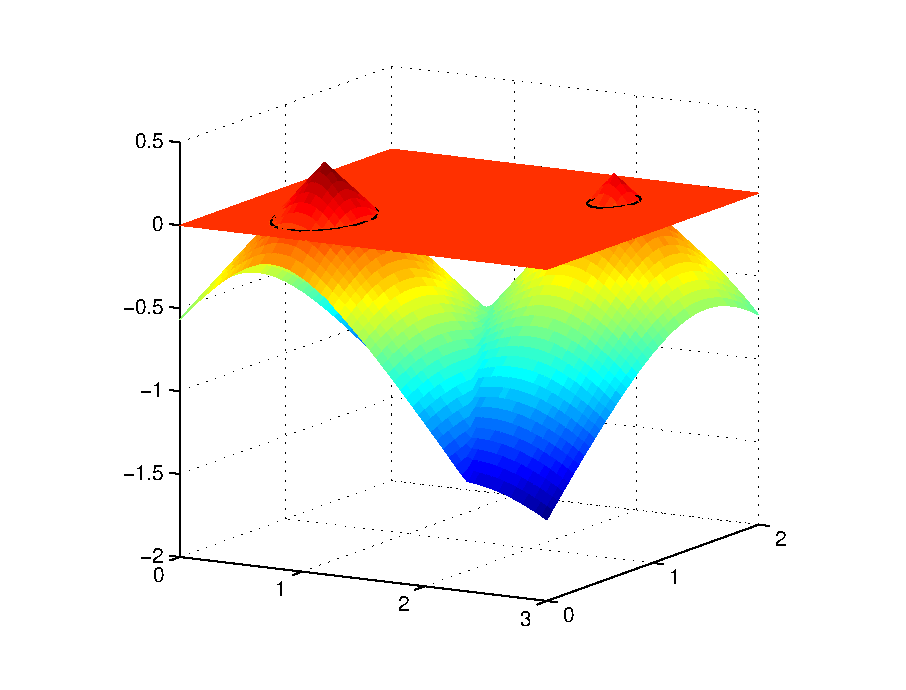
\includegraphics[width=\linewidth]{level_set_function_circles_1.eps}
		} \\
		\subfloat[]{
			\label{fig:level_set_circle_domain_050}
			\includegraphics[width=\linewidth]{level_set_circles_2.eps}
		} &
		\subfloat[]{
			\label{fig:level_set_circle_func_050}
			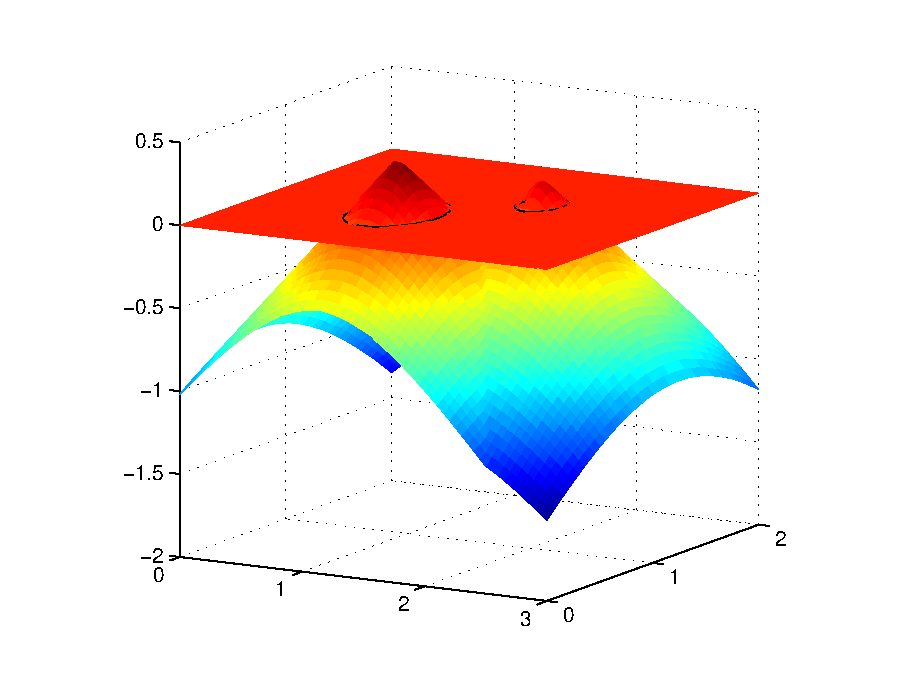
\includegraphics[width=\linewidth]{level_set_function_circles_2.eps}
		} \\
		\subfloat[]{
			\label{fig:level_set_circle_domain_075}
			\includegraphics[width=\linewidth]{level_set_circles_3.eps}
		} &
		\subfloat[]{
			\label{fig:level_set_circle_func_075}
			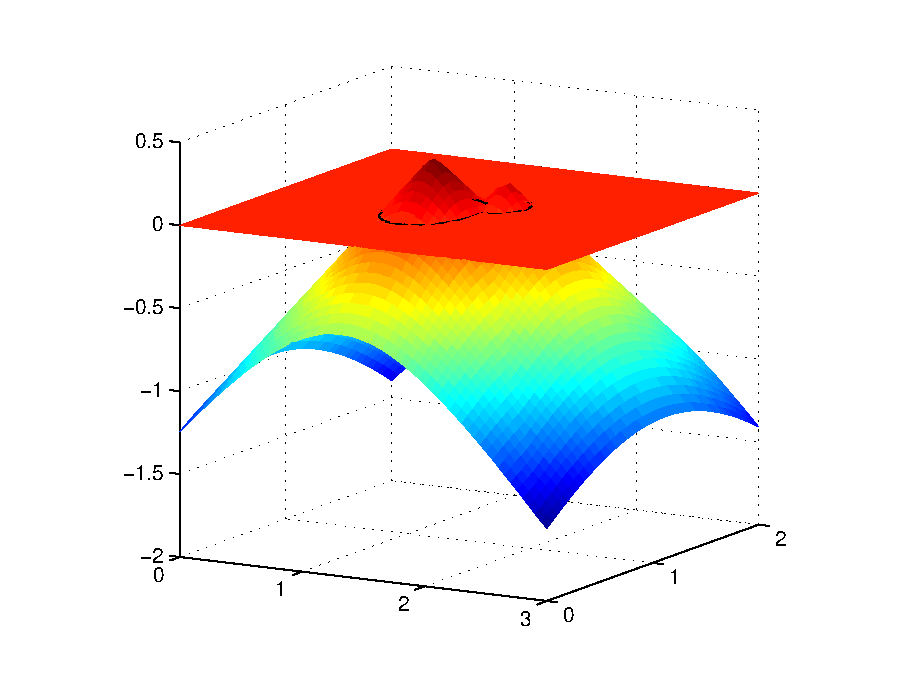
\includegraphics[width=\linewidth]{level_set_function_circles_3.eps}
		} \\
	\end{tabularx}
	\caption{Level set description of two circular inclusions with radii $0.667$ and $0.333$, respectively, moving towards each other. Level set functions can be used to describe complex topologies in a fixed mesh.}
	\label{fig:level_set_description}
\end{figure}

Multiple level set functions can be used to model more than two phase regions \ref{eq:level_set_regions}. As with the level set method itself, the use of multiple level set functions originated in image processing \citep{VC:02}. This so-called ``color'' level set method requires $m$ level set functions to model $n = 2^m$ different phase regions. For a reference on the method, the reader is referred to \citep{WW:04c,WW:05}.

The material distribution in the design domain can be determined from the phase region of the level set field. Several methods exists to describe this distribution. Density based level set methods describe the phase regions by either using element-wise constant material fractions or by mapping the level set field directly to a point \citep{YYK+:15}. These techniques are denoted as Ersatz material approaches (see Figure \ref{fig:ersatz_interpolation}) \citep{WWG:03,AJ+:05}, and while they ease the computational complexity, they lead to modeling errors. In this work, we will triangulate the element cut by the zero level set isolevel, and then perform our operations on the subdomains and on the interface (see Figure \ref{fig:XFEM_interpolation}) \citep{MM:13,VM:14}. This methodology will avoid the need to approximate material properties such as in density methods.

Regularization techniques are used in a level set optimization problem to control the geometry of the design. Among these techniques are perimeter or curvature minimization \citep{MKM+:11,YIN+:10,DLK:12}. The advantage of the level set method is that we possess a crisp definition of the phase interface, and therefore can integrate over the shape boundary $\Gamma_{\phi=0}$. These techniques will be studied in Section \ref{sec:topology_optimization_approaches_for_the_curvature_minimization_of_level_set_isocontours}.

% -----------------------------------------------------------------------------
% Topology optimization with the level set method

\subsection{Topology optimization with the level set method}

The topology of the level set field is modified by update schemes that use the sensitivities of the design variables. Several approaches exist, such as the Hamilton-Jacobi equation \citep{YNY+:10}. This work will focus on a mathematical programming approach, where the nodal values of the discrete level set field are defined as functions of the optimization design variables. Like in the filtering method of density approaches, we will define a linear filter
%
\begin{equation}
	\label{eq:smoothing_filter_XFEM}
	\phi\left(\mathbf{s}\right)=\frac{\sum_{i=1}^{N}w_{i}s_{i}}{\sum_{i=1}^{N}w_{i}}
\end{equation}

with

\begin{equation}
	\label{eq:weight_XFEM}
	w_{i}=\max \left( 0, r_{\phi} - \Vert \mathbf{x}_i - \mathbf{x} \Vert \right)
\end{equation}
%
where $\phi\left(\mathbf{s}\right)$ is the level set function at a point $\mathbf{x}$, $\mathbf{x}_{i}$ is the location of the node at which the design variable $i$ is defined, $w_{i}$ is the factor of point $\mathbf{x}$ with respect to the design variable $i$, $r_{\phi}$ is the filter radius, and $N$ is the number of nodes in the design domain. However, unlike the filter in the density approaches, this filter cannot control the minimum feature size, as discussed in Section \ref{sec:feature-size-control}.

The reader is referred to \citep{DML+:13,GP:13} for a more detailed overview of the level set method and topology optimization approaches.

% -----------------------------------------------------------------------------
% Extended finite element method

\section{Extended finite element method}
\label{sec:intro_xfem}

The extended finite element method (XFEM) is an immersed boundary technique that works on fixed meshes. The XFEM was built upon the concept of partition of unity developed by \citep{NME:NME86}, and it was originally used to model crack propagation \citep{BB:99}. Due to its ability to approximate discontinuous solutions, the method has been applied in a variety of discontinuous partial differential equations, such as multimaterial structural mechanics \citep{WW:04c,VM:14}, fluid-structure interaction \citep{GW:08}, and multi-phase flows \citep{CB:03}. The method has also been applied to shape optimization by \citep{DMJ+:06,MMF+:05,MD:07}, and to topology optimization by \citep{HMM:13,LWW:12,WWX:10,MKM+:11,MM:14,VM:14}.

The XFEM decomposes the cut elements into subdomains and interfaces that it uses to integrate the weak form of the governing equations. Figure \ref{fig:triangulation_2D} illustrates this by showing the possible decompositions of a two dimensional finite element based on its nodal level set values.
%
\begin{figure}
	\centering
	\includegraphics[width=\linewidth]{intersections_2D.eps}
	\caption{A two dimensional finite element has eight possible decompositions based on the nodal level set values.}
	\label{fig:triangulation_2D}
\end{figure}

The XFEM can model discontinuities in the solution field by augmenting the standard finite element function space with additional degrees-of-freedom, denoted ``enriched degrees-of-freedom''. To illustrate this with a quick example, consider an XFEM model that consists of a two dimensional mesh with four linear elements. The level-set distribution in Figure \ref{fig:intro_structural_model} leads to the intersection pattern shown in Figure \ref{fig:intro_physical_model}. The nodes on the left are clamped, and the right edge is subject to a constant pressure load. The node at the center of the mesh in Figure \ref{fig:intro_physical_model} will use different degrees-of-freedom to interpolate the different subdomains, and avoid artificially coupling the disconnected phase regions.
%
\begin{figure}
	\centering
	\includegraphics[width=0.75\linewidth]{structural_model.eps}
	\caption[Structural problem setup.]{Structural problem setup. The domain contains multiple level set inclusions.}
	\label{fig:intro_structural_model}
\end{figure}
%
\begin{figure}
	\centering
	\includegraphics[width=0.75\linewidth]{physical_model.eps}
	\caption[XFEM implementation example physical model]{4-element 2D mesh. Black areas: material phase 1, negative level-set value at the nodes; white areas: material phase 2, positive level-set value.}
	\label{fig:intro_physical_model}
\end{figure}

The solution space is then interpolated using the generalized enrichment formulation of \citep{HH:04}:
%
\begin{equation}
	\mathbf{u}(\mathbf{x}) = \sum \limits^{M}_{m=1} \left( H(-\phi) \sum\limits^{n}_{i=1} \mathbf{N}_i \ \mathbf{u}_{i,m}^A
														 + H( \phi) \sum\limits^{n}_{i=1} \mathbf{N}_i \ \mathbf{u}_{i,m}^B \right)
\end{equation}

where $m$ is the enrichment level, $M$ is the maximum number of enrichment levels used for each phase, $\mathbf{N}$ are the shape functions, $\mathbf{u}^l_{i,m}$ is the vector of degrees-of-freedom values at node $i$ for phase $l=[A,B]$, $\phi$ is the level set value evaluated at $\mathbf{x}$, and $H$ denotes the Heaviside function. This is illustrated in Figure \ref{fig:intro_enrichment_model} for the structural problem of Figure \ref{fig:intro_structural_model}.
%
\begin{figure}[htbp]
	\centering
	\includegraphics[width=0.9\linewidth]{enrichment_model.eps}
	\caption{The center node, denoted by the color blue, uses different degrees-of-freedom to describe the disconnected phase regions. The subscripts denote the $m$ enrichment level. The maximum number of enrichment levels used for each phase is $M=5$. A value of 0 denotes the original finite element degrees-of-freedom, while other numbers indicate additional ``enriched degrees-of-freedom''. }
	\label{fig:intro_enrichment_model}
\end{figure}

The Heaviside function $H$ depends on the level set function and is defined as follows:
%
\begin{equation}
	H(z) =
		\begin{cases}
			1 & z > 0 \\
			0 & z \le 0
		\end{cases}
\end{equation}

The Heaviside functions ``turns on/off'' the standard finite element interpolations in the particular phases. The approximation allows for discontinuities of the states $\mathbf{u}$ along the phase boundaries. Therefore, the continuity of the solution at the interface between different phase regions must be enforced. Several techniques are available in the literature, such as stabilized Lagrange multipliers (Section \ref{sec:density_and_level_set_XFEM_schemes_for_topology_optimization_of_3D_structures}) \citep{BH:10}, and the Nitsche method (Section \ref{sec:level_set_XFEM_topology_optimization_of_3D_navier_stokes_and_scalar_transport_problems}) \citep{BH:12}. More recent development include the face-oriented ghost penalty (Section \ref{sec:level_set_XFEM_topology_optimization_of_3D_navier_stokes_and_scalar_transport_problems}) by \citep{SW:14,SRG+:14,BH:12}, which aims at smoothing the gradients of the solution between cut elements. All three formulations will be studied and applied to topology optimization in this work.

For more details, refer to Sections \ref{sec:a_complete_methodology_for_the_implementation_of_XFEM_inclusive_models}, \ref{sec:discretization}, and \ref{sec:computational-considerations}. For a review of the XFEM, the user is referred to \citep{FB:10}.

% -----------------------------------------------------------------------------
% Available software

% \section{Available software}

% For the numerical modeling and simulation, we will use our in-house code, the Finite Element Multidisciplinary Optimization Code (FEMDOC). The linear algebra package is provided by Trilinos \citep{Trilinos:03}.

% -----------------------------------------------------------------------------
%
%* What is your work about?
%
%- Topology optimization approach.
%- Using the Level Set Method.
%- eXtended Finite Element Method.
%- LSM describes the geometry of the design.
%- XFEM is used to solve the PDE and measure the performance.
%- Apply methodology for complex work.
%
%* Who should care about your work?
%
%- Topology optimization community. 
%- Alternate method to homogenization methods.
%- Design engineers.
%- Surface mesh ready for three dimensional printing.
%
%* What are the goals of your thesis?
%
%- Develop robust topology optimization approach using the LSM and the XFEM methods.
%- Compare pros and cons against homogenization methods.
%- Apply methodology to real-world problem, such as ALD.
%
%* What is your overarching approach? How will you know you have accomplished your goals?
%
%- Develop methodology for triangulation, enrichment of 3D geometries (methodology section).
%- Test framework with structural problems in three dimensions (structural section).
%- Compare results with SIMP (structural section).
%- Expand to incompressible Navier-Stokes and Stokes flows, and scalar transport (fluids section).
%- Study convergence with respect to the enforcement of boundary conditions to ensure stability and coercivity.
%- Study convergence with respect to intersection configuration.
%- Study shape control and regularization techniques (curvature section).
%- Three dimensional printing (structural, fluids, curvature sections).
%- Apply methodology to ALD problem (ALD section).
%
%* Why should they care about your work?
%
%- Methodology accommodates different physics.
%- Accommodate structural, Navier-Stokes, scalar transport physics.
%- Three dimensional problems.
%- For topology optimization, it is relevant because it provides an alternate method besides homogenization methods.
%- Advantages over SIMP.
%- Explicit description of boundary for correct application of boundary conditions.
%- Regularization techniques allow shape control of the interface.
%- Prevents spurious diffusion, etc.
%- Coarser mesh leads to faster computations.
%
%* Does it enable us to solve new optimization problems or just live with coarser mesh?
%
%- Solve topology optimization problems where physics at interface is crucial.
%- ALD requires measuring temperature distribution correctly. Spurious diffusion does not help the problem.
%- Coarse mesh is good enough to describe physics at the interface.
%- In 3D, efficiency is crucial.
%
%* How is thesis proposal structured?
%
%- What sections present?
%- Mention sections are drafts of papers.